\graphicspath{{./PBL/images}}

\chapter{Projekt PBL}

Uczenie poprzez realizację projektów (ang. \angver{Project Based Learning}, PBL) jest metodą uczenia 

\section{Cel projektu} \label{cel_projektu}

Celem wspomnianego projektu było zaprojektowanie układu laboratoryjnego, składającego się z klatki Helmholtza oraz umieszczonego wewnątrz klinostatu trójwymiarowego. Docelowo taki układ pozwalałby na przeprowadzanie badań nad rozwojem roślin w warunkach symulowanej mikrograwitacji bez ziemskiego pola magnetycznego. Klatka Helmholtza jest złożeniem trzech par cewek Helmholtza w takiej konfiguracji aby osie magnetyczne każdej z par było prostopadłe do pozostałych. Pozwala to wytworzyć wektor indukjcji magnetycznej o dowolnym kierunku przestrzennym i bardzo wysokiej jednorodności. Wysoka jednorodność jest kluczowa aby generowany wektor indukcji magnetycznej był stały w objętości przeprowadzanego eksperymentu. W związku z wymaganiami projektu, wewnętrzna konstrukcja klinostatu musiała zostać wykonana tak, aby mieć jak najmniejszy wpływ na panujące wewnątrz warunki magnetyczne. Naturalnie rodzi to zagadnienie wyboru materiałów konstrukcyjnych klinostatu, które nie powinny mieć właściwości ferromagnetycznych, powinny mieć względnie niską przewodność elektryczną w celu eliminacji indukowanych prądów wirowych oraz dodatkowym ich atutem będzie niska podatność magnetyczna. Oprócz właściwości magnetycznych materiałów istnotne są też możliwości ich obróbki termicznej oraz mechanicznej, a również ich forma, co później ma wpływ na prostotę montażu urządzenia. Oprócz samych wymagań materiałowych oraz konstrukcyjnych, należało również zapewnić optymalne warunki wzrostowe obiektów badawczych, należało określić odpowiedni rozmiar cewek, aby objętość o wysokim stopniu jednorodności magnetycznej była odpowiednio duża oraz wiele innych. Taki szereg wymagań stworzył bardzo ciekawe i multidyscyplinarne wyzwanie inżynieryjne, które wymagało użycia oraz w niektórych przypadkach stworzenia wielu środowisk symulacyjnych w celu jego rozwiązania. Projekt wykonywany był w zespole 5-cio osobowym na przestrzeni jednego semestru. Cały model komputerowy układu klinostatu wraz z klatką Helmholtza przedstawiony został na Rys. \ref{fig:klatka_helmholtza}.

\begin{figure}
	\centering
	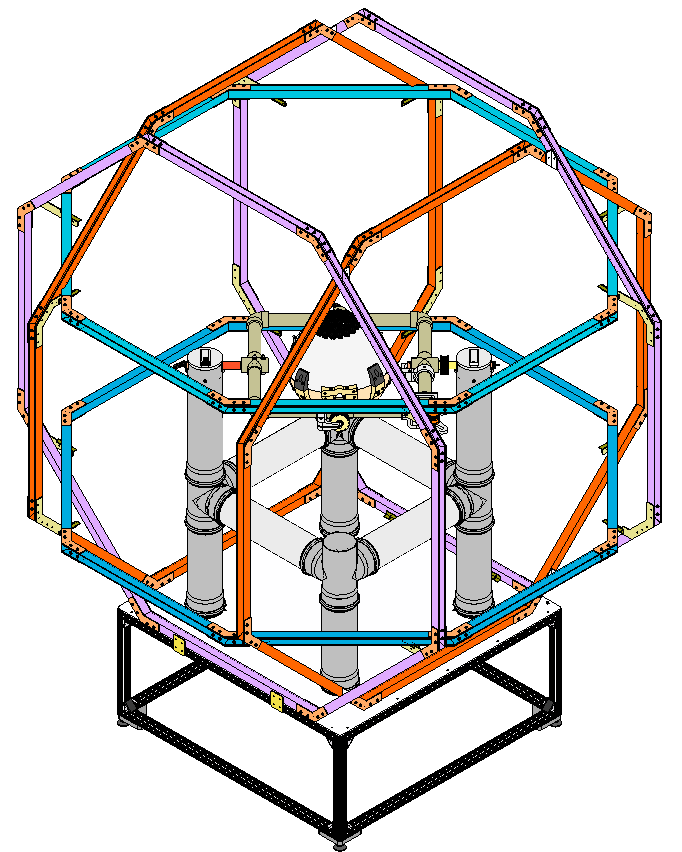
\includegraphics[scale=0.5]{klinostat_klatka}
	\caption{Projekt klatki Helmholtza z klinostatem.} 
	\caption*{Źródło: opracowanie własne}
	\label{fig:klatka_helmholtza}
\end{figure}

\section{Konstrukcja klinostatu}

Ten podrozdział poświęcony został krótkiemu opisowi konstrukcji samego klinostatu zaprojektowanego w ramach PBL. Zaprojektowane urządzenie jest klinostatem o dwóch stopniach swobody, każdy stopień posiada swój osobny napęd. Oznacza to iż jest to maszyna RPM, natomiast jest możliwość uruchomienia go w trybach klinostatu 2-D oraz 3-D jak opisano w podrozdziale \ref{klinostat3d}. Zewnętrzna rama klinostatu wykonana została z rur polipropylenowych (PP) stabilizowanych włóknem szklanym. Odcinki rur wraz z kształtkami 90$^\circ$ oraz czwórnikami zostały połączone metodą polifuzji termicznej (zgrzewanie). Tego typu rury wykorzystywane są w instalacjach centralnego ogrzewania, dzięki czemu ich koszt jest niski. Przeprowadzone analizy elementów skończonych (FEM), wskazały iż materiał ten posiada wystarczającą wytrzymałość aby wykorzystać go jako element strukturalny ramy klinostatu. Jako wał obrotowy wykorzystano rurę aluminiową o średnicy $PODAĆ$. Wykorzystanie łożysk kulowych w konstrukcji klinostatu nie było wskazane ze względu na wymagania opisane w podrozdziale \ref{cel_projektu}. Z tego powodu każdy z interfejsów obrotowych stanowiły tuleje ślizgowe wykonane z materiału iglidur, zaprojektowanego przez firmę IGUS.



\section{Modyfikacje projektu}

\section{Napęd klinostatu}

\section{Elektronika układu sterowania}